\documentclass[a4paper,14pt]{extreport}
\newlength{\curtextsize}
\makeatletter 
\setlength{\curtextsize}{\f@size pt}
\makeatother
\usepackage{polyglossia}
\setdefaultlanguage{russian}
\setotherlanguages{english,german}
\usepackage[labelsep=period, nooneline]{caption} % Заменить умолчальное разделение ':' на '.'в подписях к рисункам и таблицам
\defaultfontfeatures{Mapping=tex-text}% Для работы кавычек, тире и т.д.
%\setmainfont{Times New Roman} % Основной шрифт документа
%\setmainfont{CharterITC}
\setmainfont{CMU Serif Roman}
\newfontfamily{\cyrillicfonttt}{CMU Serif Roman}

%Поиск в пдф-документе
\usepackage{cmap}

% Пакеты для xelatex
\usepackage{xunicode, xltxtra}

% Работа с геометрией страницы
\usepackage{geometry}

% Дополнительная работа с математикой
\usepackage{mathtext} % Русские буквы в формулах
\usepackage{amsmath, amssymb, amsthm, amsfonts, mathtools} % AMS
\usepackage{icomma} % "Умная" запятая: $0,2$ --- число, $0, 2$ --- перечисление

% Шрифты
\usepackage{euscript} % Шрифт Евклид
\usepackage{mathrsfs} % Красивый матшрифт

% Пакеты для работы с таблицами
\usepackage{verbatim, array, booktabs, multirow, makecell, tabu, longtable, xcolor, colortbl, wrapfig}

% Для печати в несколько колонок
\usepackage{multicol}

% Для двойной горизонтальной линии в таблицах
\usepackage{hhline}

% Для подключения eps графики
\usepackage{epstopdf}

% Для пробелов в названиях и путях к картинкам
\usepackage{graphicx}
\usepackage[space]{grffile}

% Неразобранные, но нужные пакеты (подключались по мере необходимости для выполнения разных задач)
\usepackage{titletoc, rotating, fp, fontspec, setspace, cite, tikz, tocloft, ifpdf, kvoptions, subfig, latexsym, listings, pgfplots, pgfpages, xifthen, ulem, float, indentfirst, enumerate, titlesec, enumitem, todonotes, lettrine, lipsum, pdflscape, pdfpages, ragged2e, lastpage, etoolbox}

% Библиотеки для графического пакета tikz
\usetikzlibrary{intersections, fit, automata, calc, trees, positioning, arrows, chains, shapes.geometric, decorations.pathreplacing, decorations.pathmorphing, shapes, matrix, shapes.symbols, shadows, backgrounds, mindmap, shapes.gates.logic.US, trees, positioning, circuits.logic.IEC, shapes.gates.logic.IEC, shapes.geometric
}

% Подключаем графический пакет для рисования диаграмм
\usepgfmodule{plot}

% Задаем геометрию полей страницы
\geometry{left=2cm}
\geometry{right=1cm}
\geometry{top=2cm}
\geometry{bottom=2cm}

% Заменяем вводимые с клавиатуры кавычки на елочки
\usepackage{csquotes}
%\MakeOuterQuote{"}



% Названия глав располагаем с красной строки и устанавливаем их размер и отступы до и после названия
\makeatletter
%\def\section{\@dblarg\@section}
%\def\@section[#1]#2{\refstepcounter{section}%
%        \vspace{28pt plus 1cm minus 7pt}\par\pagebreak[3]%
%        \hangindent=\parindent
%        {\nobreak\noindent\hspace*{\hangindent}\raggedright\bf
%        \llap{\thesection\space}\lowercase{#2}}%
%        \addcontentsline{toc}{section}{\thesection\space #1}\par\nobreak}
%
%\def\section{\@dblarg\@section}
%\def\@section[#1]#2{\refstepcounter{section}%
%        {\newpage\nobreak\hspace*{.5cm}\raggedright
%        \llap{\thesection\space\space}\uppercase{#2}}%
%        \addcontentsline{toc}{section}{\thesection\space #1}\par\nobreak}

\def\section{\@dblarg\@section}
\def\@section[#1]#2{\refstepcounter{section}%
        {\newpage\nobreak\hspace*{.5cm}\raggedright
        \llap{\thesection\space\space}\uppercase{#2}}%
        \addcontentsline{toc}{section}{\thesection\space #1}\par\nobreak}
\renewcommand{\subsection}[1]{\refstepcounter{subsection}
        \vspace{15pt plus 7pt minus 3pt}\nobreak\par%
        {\thesubsection\space #1}%
        \addcontentsline{toc}{subsection}{\thesubsection\space #1}%
        \par\vspace{2ex}}
\renewcommand{\subsubsection}[1]{\refstepcounter{subsubsection}
        \vspace{15pt plus 7pt minus 3pt}\nobreak\par%
        {\thesubsubsection\space #1}%
        \addcontentsline{toc}{subsubsection}{\thesubsubsection\space #1}%
        \par\vspace{2ex}}

\makeatother

% Ставим или убираем номера глав

%\makeatletter
%\renewcommand\thechapter{\@arabic\c@chapter}
%\renewcommand\thesection{\@arabic\c@section}
%\gappto\russian@capsformat{\renewcommand{\postsection}{\@aftersepkern}}
%\renewcommand\thesubsection{\@arabic\c@section.\@arabic\c@subsection}
%\gappto\russian@capsformat{\renewcommand{\postsubsection}{\@aftersepkern}}
%\renewcommand\thesubsubsection{\@arabic\c@section.\@arabic\c@subsection.\@arabic\c@subsubsection}
%\gappto\russian@capsformat{\renewcommand{\postsubsubsection}{\@aftersepkern}}
%\makeatother

\newcounter{secnum}

\setcounter{secnum}{2}

\ifnumequal{\value{secnum}}{1}{%
% Убираем точки после цифры в главах и подглавах
\renewcommand\thechapter{\arabic{chapter}}
\renewcommand\thesection{\arabic{section}}
\renewcommand\thesubsection{\arabic{section}.\arabic{subsection}}
\renewcommand\thesubsubsection{\arabic{section}.\arabic{subsection}.\arabic{subsubsection}}
}{}

\ifnumequal{\value{secnum}}{2}{%
% Убираем точки после цифры в главах и подглавах
\renewcommand\thechapter{}
\renewcommand\thesection{}
\renewcommand\thesubsection{}
\renewcommand\thesubsubsection{}
}{}

% Задаем отступ от нумерации названия глав и подглав в Содержании
\makeatletter
\newcommand{\l@likechapter}{\@dottedtocline{1}{1em}{1em}}
\renewcommand{\l@chapter}{\@dottedtocline{1}{1em}{1em}}
\renewcommand*\l@section{\@dottedtocline{1}{1em}{1em}}%
\renewcommand*\l@subsection{\@dottedtocline{1}{2.0em}{1.7em}}%
\renewcommand*\l@subsubsection{\@dottedtocline{1}{3.6em}{2.4em}}%
\newcommand*\l@subsubsubsection{\@dottedtocline{1}{6em}{2.4em}}%
\makeatother

% Настройка Содержания
\gappto\captionsrussian{\renewcommand{\contentsname}{Оглавление}}
\renewcommand{\cfttoctitlefont}{\hspace{0.38\textwidth}\MakeUppercase
}
\renewcommand{\cftbeforetoctitleskip}{-2em}% Отступ от верхнего края до Содержания
\renewcommand{\cftaftertoctitle}{\mbox{}\hfill \\ \mbox{}\hfill{}\vspace{-2.5em}}% Отступ от Содержания до текста

% Запрещаем переносы в Содержании
\makeatletter
\renewcommand{\@tocrmarg}{2.55em plus1fil}
\makeatother
\setcounter{secnumdepth}{3} % глубина глав 2 (чаптер, секшн, субсекшн)
\setcounter{tocdepth}{3} % глубина оглавления

% Обозначения и сокращения
\usepackage[russian]{nomencl}
\newcommand{\nomdescr}[1]{{--\hskip0.7cm}\parbox[t]{15cm}{\RaggedRight #1}}
\newcommand{\nomwithdim}[3]{\nomenclature[#1]{#2}{\nomdescr{#3}}}
\newcommand{\nom}[3][]{\nomwithdim{R#1}{#2}{#3}}
\makenomenclature
\renewcommand{\nomname}{%
\vspace{-3.5cm}
\centerline{%
\normalfont
\normalsize
\MakeUppercase{\textmd{Список сокращений и условных обозначений}}
}
\vspace{-0.5cm}
}
\setlength{\nomitemsep}{-0.25cm}

% Определяем кавычки <<елочки>>
\DeclareQuoteStyle{russian}
{\guillemotleft}{\guillemotright}[0.025em]
{\quotedblbase}{\textquotedblleft}
\ExecuteQuoteOptions{style=russian}
\newcommand{\elki}[1]{\enquote{#1}}

% Списки --, 1. и а) с отступом первой строки
% Нумерация + вложенная нумерация
\renewcommand{\alph}[1]{\asbuk{#1}} 
\setlist{nolistsep}
\setitemize[1]{label=--, fullwidth, itemindent=\parindent, listparindent=\parindent}
\setitemize[2]{label=--, fullwidth, itemindent=\parindent, listparindent=\parindent, leftmargin=\parindent}
\setitemize[3]{label=--, fullwidth, itemindent=\parindent, listparindent=\parindent, leftmargin=\parindent}
\setenumerate[1]{label=\arabic*., fullwidth, itemindent=\parindent, listparindent=\parindent}
\setenumerate[2]{label=\arabic{enumi}.\arabic{enumii}, fullwidth, itemindent=\parindent, listparindent=\parindent, leftmargin=\parindent}
\setenumerate[3]{label=\arabic{enumi}.\arabic{enumii}.\arabic{enumiii}, fullwidth, itemindent=\parindent, listparindent=\parindent, leftmargin=\parindent}
\setenumerate[4]{label=\alph*), fullwidth, itemindent=\parindent, 
listparindent=\parindent, leftmargin=\parindent}

% Формат подрисуночной (табличной, формульной) надписи и их нумерация
\makeatletter
\@addtoreset{table}{section}
\@addtoreset{figure}{section}
\makeatother
\addto\captionsrussian{\def\figurename{Рисунок}
\renewcommand{\tablename}{Таблица}}
\renewcommand{\thefigure}{\thesection.\arabic{figure}}
\renewcommand{\thetable}{\thesection.\arabic{table}}
\renewcommand{\theequation}{\thesection.\arabic{equation}}
%\setlength{\intextsep}{5mm}%Увеличиваем расстояние между основным текстом и рисунком под ним
%\setlength\belowcaptionskip{-5mm}%Уменьшаем расстояние между основным текстом и рисунком над ним
\RequirePackage{caption}
\DeclareCaptionLabelFormat{fullparens}{\bothIfFirst{#1}{~}#2}
\captionsetup[figure]{
format=plain,
indention=0.7cm,
justification=centering,
labelsep=endash,
skip=5mm
}
\captionsetup[table]{
format=plain,
font={footnotesize},
labelformat=fullparens,
labelsep=endash,
%labelfont=it,
%textfont=bf,
justification=raggedright,
singlelinecheck=false
}
\makeatletter
\setlength\abovecaptionskip{2\p@}
\setlength\belowcaptionskip{1\p@}
\makeatother

% Убираем связанность номера формулы с номером главы/раздела 0 --- есть зависимость от номера главы, 1 --- нет.
\newcounter{contnumfig}

\setcounter{contnumfig}{1}

\ifnumequal{\value{contnumfig}}{1}{%
\renewcommand{\thefigure}{\arabic{figure}}
\renewcommand{\thetable}{\arabic{table}}
\renewcommand{\theequation}{\arabic{equation}}
}{}

% Переопределение списков itemize и enumerate, убирающее расстояния между строками и абзацами
\makeatletter
\renewcommand{\@listI}{%
\topsep=0pt }
\makeatother

\makeatletter
\let\old@itemize=\itemize
\def\itemize{\old@itemize
\setlength{\itemsep}{0pt}
\setlength{\parskip}{0pt}
\setlength{\leftskip}{0pt}
}
\makeatother

\makeatletter
\let\old@enumerate=\enumerate
\def\enumerate{\old@enumerate
\setlength{\itemsep}{0pt}
\setlength{\parskip}{0pt}
\setlength{\leftskip}{0pt}
}
\makeatother


%%% Определение subsubsubsection
\makeatletter
\newcommand{\subsubsubsection}[1]{\refstepcounter{subsubsubsection}
        \vspace{15pt plus 7pt minus 3pt}\nobreak\par%
        {\thesubsubsubsection\space #1}%
        \addcontentsline{toc}{subsubsubsection}{\thesubsubsubsection\space #1}%
        \par\vspace{2ex}}
\newcounter {subsubsubsection}[subsubsection]

\renewcommand\thesubsubsubsection{\thesubsubsection .\@arabic\c@subsubsubsection}
 \makeatother
 


% Работа с датой
\usepackage[ddmmyyyy]{datetime}
\renewcommand{\dateseparator}{.}
\def\daterussian{%
\def\mon{\ifcase\month\or января\or февраля\or марта 
\or апреля\or мая\or июня\or июля\or августа\or сентября 
\or октября\or ноября\or декабря\fi\space}%
}



% Создание счетчиков страниц, разделов, рисунков, таблиц, приложений
\usepackage[square,numbers,sort&compress]{natbib}

\newcounter{reference}
\pretocmd{\bibitem}{\addtocounter{reference}{1}}{}{}

\usepackage[chapter,     %
            page,         %
            section,     %
            figure,      %
            table,       %
            reference,   %
            ]{totalcount}

% Оставил этот пример. Из него можно вытянуть дополнительные счетчики, если они понадобятся (например можно сделать счетчик чего-то в документе отдельно от приложений)
%\newcounter{totfigures}
%\newcounter{tottables}
%\newcounter{totsections}
%\newcounter{totreferences}
%\newcounter{totchapter}
%\makeatletter
%\AtEndDocument{%
%\addtocounter{totsections}{\value{section}}%
%\addtocounter{totfigures}{\value{figure}}%
%\addtocounter{tottables}{\value{table}}%
%\addtocounter{totchapter}{\value{chapter}}%
%\immediate\write\@mainaux{%
%\string\gdef\string\totsec{\number\value{totsections}}%
%\string\gdef\string\totfig{\number\value{totfigures}}%
%\string\gdef\string\tottab{\number\value{tottables}}%
%\string\gdef\string\totref{\number\value{totreferences}}%
%\string\gdef\string\totpril{\number\value{totchapter}}%
%}%
%}
%\makeatother
%\pretocmd{\section}{\addtocounter{totfigures}{\value{figure}}}{}{}
%\pretocmd{\section}{\addtocounter{tottables}{\value{table}}}{}{}
%\pretocmd{\chapter}{\addtocounter{totfigures}{\value{figure}}}{}{}
%\pretocmd{\chapter}{\addtocounter{tottables}{\value{table}}}{}{}
%\pretocmd{\bibitem}{\addtocounter{totreferences}{1}}{}{}
%\pretocmd{\chapter}{\addtocounter{totchapter}{0}}{}{}
%\pretocmd{\section}{\addtocounter{totsections}{1}}{}{}% При включении Приложения раскомментировать


% Создание своего оформления для произвольной главы
\newcommand{\empline}{\mbox{}\newline}
\newcommand{\likechapter}[1]{
\newpage
\begin{center}
\MakeUppercase{#1}
\end{center}
\vspace{-1cm}
\empline}



% Настройка Приложений
\usepackage[title,titletoc]{appendix}
%\newcommand{\empline}{\mbox{}\newline} % пустая строка
\newcommand{\append}[1]{%
    \clearpage
    \refstepcounter{chapter}
    \begin{center}
       \MakeUppercase{%
       \appendixname~\Asbuk{chapter}}
    \end{center}
    \begin{center}{#1}\end{center}
    \renewcommand{\thefigure}{\Asbuk{chapter}.\arabic{figure}}
	\renewcommand{\thetable}{\Asbuk{chapter}.\arabic{table}}
	\renewcommand{\theequation}{\Asbuk{chapter}.\arabic{equation}}
	\renewcommand{\thesubsection}{\Asbuk{chapter}.\arabic{subsection}}
	\renewcommand{\thesubsubsection}{\Asbuk{chapter}.\arabic{subsection}.\arabic{subsubsection}}
	\renewcommand{\thesubsubsubsection}{\Asbuk{chapter}.\arabic{subsection}.\arabic{subsubsection}.\arabic{subsubsubsection}}
    \empline
    %В приложениях эта строка вставлена, поэтому здесь коментим
    %\addcontentsline{toc}{chapter}{\Asbuk{chapter}\hspace{0em}~#1}
    }


% Создание примечания зеленым
\newcommand{\prim}{\todo[color=green!40,inline,caption={\textit{Примечание}}]}

% Тодо делаем красным
\DeclareRobustCommand{\todo}{\textcolor{red}}

%Переносы вкл. и 1.5 интервала выкл.
\newcommand{\pereodin}{\hyphenpenalty=100\singlespacing}

%%% Настройка библиографии
\makeatletter
%Стиль библиографических ссылок БибТеХа - нумеровать в порядке упоминания в тексте
\bibliographystyle{%
%ugost2008%
BibTeX-Styles/ugost2008%
%BibTeX-Styles/utf8gost71u%
}
%Заменяем квадратные скобки в списке литературы на цифру без точки, если нужна точка, то ставим ее после {#1.}
\renewcommand{\@biblabel}[1]{#1}
\makeatother
\newcommand\mybibname{Список использованных источников}
% bibsection используется в пакете natbib
\renewcommand\bibsection{%
\newpage\centering\vskip2cm
\noindent\normalsize\MakeUppercase{\mybibname}%
\markboth{\MakeUppercase{\mybibname}}{\MakeUppercase{\mybibname}}%
\addcontentsline{toc}{section}{Список использованных источников}
\vskip1cm}

\sloppy%Перенос слов, которые не убираются в строке (вылезают на поля)
\clubpenalty=10000 % Запрещаем разрыв страницы после первой строки абзаца
\widowpenalty=10000 % Запрещаем разрыв страницы после последней строки абзаца
\brokenpenalty=10000 % Подавление переносов на другую страницу
\hyphenpenalty=10000 % Запрещаем переносы
\parfillskip=0pt plus .95\textwidth % Последняя строка абзаца не будет слишком короткой
\parindent=1cm% Абзацный отступ
%\renewcommand{\baselinestretch}{1.3}% Межстрочный интервал
\onehalfspacing
\renewcommand{\ge}{\geqslant}
\renewcommand{\le}{\leqslant}
\righthyphenmin=2 % Минимальное число символов при переносе - 2.
\tabulinesep=1mm%Расстояние между нижней чертой и содержимым в ячейке таблицы
\newcommand\marker[2]{{\fboxsep=0pt\colorbox{green!50}{\strut }}}
\usepackage{hyperref}
\usepackage{hyperxmp}
\hypersetup
{
    pdfauthor={User},
    pdfcreator={Microsoft® Word 2010},
    pdfproducer={Microsoft® Word 2010}
}
\usepackage{fancyhdr}

%%% Переопределяем шрифт в заголовках таблиц
%\renewcommand\theadset{\def\arraystretch{.75}}
\renewcommand\theadfont{\bfseries\footnotesize}
%%% Уменьшаем вертикальные расстояния в заголовках таблиц сверху и снизу от подписи
\renewcommand\theadgape{\Gape[0pt][0pt]}

%%% Временно
\makeatletter
\newcommand{\verbatimfont}[1]{\renewcommand{\verbatim@font}{\ttfamily#1}}
\makeatother

%%%%%%%%%%%%%%%%%%%%%%%%%%%%%%%%%
%red, green, blue, cyan , magenta, yellow, black, gray, darkgray, lightgray, brown, lime, olive, orange, pink, purple, teal, violet, white.
\tikzset{
skip loop/.style={
to path={-- ++(0,-.5) -| (\tikztotarget)}
},
skip loop1/.style={
to path={-- ++(0,-.8) -| (\tikztotarget)}
},
every annotation/.style={%Это аннотация для диаграммы дерева
fill=red!20
},
%root concept/.append style={%Это родительский круг, основа
%concept,
%circular drop shadow,
%font=\footnotesize,
%concept color=black!100,
%fill=black!05,
%line width=1ex,
%text=black,
%minimum size=3cm
%},
%level 1 concept/.append style={%Это дочерний кружок 1 уровня, т.е. первый от родительского
%every child/.style={
%},
%concept,
%circular drop shadow,
%%concept color=blue!60!violet!40,
%font=\scriptsize,
%fill=black!05,
%line width=1ex,
%text=black,
%level distance=45mm,%Расстояние между узлами
%minimum size=1cm
%},
%level 2 concept/.append style={%Это дочерний кружок 2 уровня, т.е. первый от родительского
%every child/.style={
%},
%concept,
%%circular drop shadow,
%font=\scriptsize,
%concept color=white!20!orange!50,
%fill=white,
%line width=0.5ex,
%text=black,
%%clockwise from=180,%По часовой стрелке, начиная от 180 градусов
%%sibling angle=30,%Дочерний угол (между кружками) 30 градусов
%level distance=27mm,%Расстояние между узлами
%minimum size=0.5cm
%},
background rectangle/.style=
{draw=black!80,
very thick,
dashed,
rounded corners
},
gkw/.style={rounded corners,fill=green!10!white,text width=11cm,align=justify},
rkw/.style={rounded corners,fill=red!10!white,text width=11cm,align=justify},
bkw/.style={rounded corners,fill=blue!10!white,text width=11cm,align=justify},
block0/.style={%Это полный желтый прямоугольник
	rounded corners,
	draw=black!80,
	top color=white,
	bottom color=yellow!50!black!20,
	very thick,
	drop shadow,
	font=\footnotesize,
	text centered,
	minimum height=2.3cm,
	minimum width=2cm,
	text width=2.5cm,
	inner sep=2mm
},
blockcl/.style={%Это полный  прямоугольник без заливки
% rounded corners,
	draw=black!80,
	very thick,
	font=\footnotesize,
	text centered,
	minimum height=2.3cm,
	minimum width=2cm,
	text width=2.5cm,
	inner sep=2mm
},
block/.style={%Это полный голубой прямоугольник
	rounded corners,
	draw=black!80,
	top color=white,
	bottom color=blue!50!black!20,
	very thick,
	drop shadow,
	font=\footnotesize,
	text centered,
	minimum height=2.3cm,
	minimum width=2cm,
	text width=2.5cm,
	inner sep=2mm
},
blockp/.style={%Это пустой прямоугольник
	very thick,
	font=\footnotesize,
	text centered,
	minimum height=2.3cm,
	minimum width=2cm,
	text width=2.5cm,
	inner sep=2mm
},
blockbukv/.style={%Это прямоугольник-буквица
	rounded corners,
	draw=black!80,
	top color=white,
	bottom color=blue!50!black!20,
	very thick,
	font=\footnotesize,
	text centered,
	minimum height=2.3cm,
	minimum width=2cm,
	text width=2.5cm,
	inner sep=2mm
},
blockt/.style={
	node distance=5mm and 55mm,
	align=center,
	on chain,
	on grid,
	rounded corners,
	draw=black!80,
	top color=white,
	bottom color=blue!50!black!20,
	very thick,
	drop shadow,
	font=\footnotesize,
	text centered,
	minimum height=2.3cm,
	minimum width=2cm,
	text width=4cm,
	inner sep=2mm
},
block1/.style={
	rounded corners,
	draw=black!80,
	top color=white,
	bottom color=green!50!black!20,
	very thick,
	drop shadow,
	font=\footnotesize,
	text centered,
	minimum height=2.3cm,
	minimum width=2cm,
	text width=2.5cm,
	inner sep=2mm
},
block2/.style={
	rounded corners,
	draw=black!80,
	top color=white,
	bottom color=orange!50!black!20,
	very thick,
	drop shadow,
	font=\footnotesize,
	text centered,
	minimum height=2.3cm,
	minimum width=2cm,
	text width=2.5cm,
	inner sep=2mm
},
dblock/.style={
	node distance=5mm,
	on chain,
	on grid,
	diamond,
	aspect=2,
	draw=black!80,
	top color=white,
	bottom color=orange!50!black!20,
	very thick,
	drop shadow,
	font=\footnotesize,
	text centered,
	minimum height=2.3cm,
	minimum width=2cm,
	text width=2.5cm,
	inner sep=2mm
},
cblock/.style={
	circle,
	draw=black!80,
	left color=green!60!blue!50,
	right color=orange!80!blue!50,
	very thick,
	drop shadow,
	font=\Large,
	text centered,
	minimum height=2.3cm,
	minimum width=2cm,
	text width=2.5cm,
	inner sep=2mm
},
line/.style={-latex,draw,rounded corners,thick},
line_plain/.style={draw,rounded corners,thick},
every join/.style={line},
line dec/.style={decoration={pre length=#1,post length=#1}},
}


\begin{document}

%\section{Математические модели взаимодействия приложения с алгоритмами синхронизации}
%
%\subsection{Взаимодействие приложения со строго синхронным АС}
%
%\begin{equation}
%\label{eq:АС с синхронизацией взаимодействий}
%\left\{
%\begin{aligned}
%x_{i+1}^n & = \begin{cases}
% x_{i}^n = x_i^n + \xi_i^n, & \text{если $x_i^n=X_i$} \\
% x_{i}^n, & \text{иначе}
% \end{cases}\\
%X_{i+1}^n & = \min\limits_{n=\overline{1,N}}(x_{i+1}^n)\\
%x_{0}^n&=0\\
%X_{0}^n&=0\\
%n & = \overline{1, N}
%\end{aligned}
%\right.
%\end{equation}
%
%\begin{figure}[H]
%\centering
%\includegraphics[scale=0.65]{графика/1.1.png}
%
%\caption{Продвижение времени}
%\label{fig:выполнение модели}
%\end{figure}
%
%
%\begin{figure}[H]
%\centering
%\includegraphics[scale=0.7]{графика/1.2.png}
%
%\caption{Продвижение времени}
%\label{fig:выполнение модели}
%\end{figure}
%
%\subsection{Взаимодействие приложения с консервативным АС}
%
%\begin{equation}
%\label{eq:АС с синхронизацией взаимодействий}
%\left\{
%\begin{aligned}
%x_{i+1}^n & = x_i^n + \xi_i^n F^n(i)\\
%F^n(i) & = \begin{cases}
% 1, & \text{если $\forall m \in M^n : x_i^n + \xi_i^n \leqslant x_i^m + \xi_i^m$} \\
% 0, & \text{иначе}
% \end{cases}\\
%x_0^n & = 0\\
%n & = \overline{1, N}
%\end{aligned}
%\right.
%\end{equation}
%
%\begin{figure}[H]
%\centering
%\includegraphics[scale=0.65]{графика/2.1.png}
%
%\caption{Продвижение времени}
%\label{fig:выполнение модели}
%\end{figure}
%
%
%\begin{figure}[H]
%\centering
%\includegraphics[scale=0.65]{графика/2.2.png}
%
%\caption{Продвижение времени}
%\label{fig:выполнение модели}
%\end{figure}
%
%
%\subsection{Взаимодействие приложения с оптимистическим АС}
%
%\begin{equation}
%\label{eq:АС с синхронизацией взаимодействий}
%\left\{
%\begin{aligned}
%x_{i+1}^n & = x_i^n + \xi_i^n-\max\limits_{m=\overline{1, N}}((x_i^n-x_i^m)I_i^{m\rightarrow n}I_i^{x_i^m<x_i^n})\\
%x_0^n & = 0\\
%n & = \overline{1, N}
%\end{aligned}
%\right.
%\end{equation}
%
%\begin{figure}[H]
%\centering
%\includegraphics[scale=0.65]{графика/3.1.png}
%
%\caption{Продвижение времени}
%\label{fig:выполнение модели}
%\end{figure}
%
%
%\begin{figure}[H]
%\centering
%\includegraphics[scale=0.65]{графика/3.2.png}
%
%\caption{Продвижение времени}
%\label{fig:выполнение модели}
%\end{figure}
%
%Вывод:
%Согласно выдвинутого ранее критерия эффективности АС, лучшим для данного приложения (модели) является тот АС, который быстрее других продвигает её модельное время.
%
%В результате проведенных экспериментов с моделями взаимодействия исследуемого приложения с алгоритмами синхронизации, можно сделать вывод, что лучшим среди исследованных строго синхронного, консервативного и оптимистического АС является последний, т.к. продвигает модельное время на большую, чем остальные АС величину.
\likechapter{Алгоритм выбора оптимальной синхронизации процессов в распределенной имитационной системе}

Благодаря интенсивному развитию вычислительной техники моделирование приобретает общенаучный характер и применяется в исследованиях объектов и процессов, происходящих в природе, в науках о человеке и обществе.

Одним из наиболее важных применений моделей в практическом, и в историческом аспектах является прогнозирование поведения моделируемых объектов.

Моделирование применяется сегодня в самых различных областях: экологии и геофизике (анализ распространения загрязняющих веществ в атмосфере), транспорте (конструирование транспортных средств, полетные имитаторы для тренировки пилотов), электронике и электротехнике (эмуляция работы электронных устройств), экономике и финансах (прогнозирование цен на финансовых рынках), архитектуре и строительстве (исследование поведения зданий, конструкций и деталей под механической нагрузкой), управлении и бизнесе (моделирование рынков сбыта и рынков сырья), промышленности (моделирование роботов и автоматических манипуляторов), медицине и биологии (моделирование пандемий и эпидемий), политике и военном деле (моделирование развития межгосударственных отношений, моделирование театра военных действий).


Применение моделей позволяет проводить контролируемые эксперименты в тех ситуациях, где экспериментирование на реальных объектах было бы практически невозможным или экономически нецелесообразным.~\cite{Shennon} В таких случаях может быть построена модель, на которой необходимые эксперименты могут быть проведены с относительной легкостью и недорого.

%Непосредственное экспериментирование с системой обычно состоит в варьировании её некоторых параметров. При этом, поддерживая все остальные параметры неизменными, наблюдают результаты эксперимента.  

%Зачастую моделирование используется в тех случаях, когда исследование процесса невозможно или невыгодно по определенным причинам, например, это может быть высокая стоимость создания процесса, его сложное строение, небольшие пространственно-временные размеры и т.д.

Выделяют три основных вида моделирования: аналитическое, численное и имитационное \cite{disksobmod}. В данной работе речь пойдет о имитационном моделировании. Имитационное моделирование --- моделирование, при котором моделирующий алгоритм с той или иной степень точности воспроизводит функционирование исходной системы. Имитационная модель воспроизводит поведение моделируемой системы во времени. Имитационная модель может быть выполнена на распределенной вычислительной системе, где выигрыш по времени выполнения модели достигается за счет параллельного выполнения событий, запланированных на разные моменты модельного времени.

Существует несколько технологий на уровне архитектур, которые позволяют задать основные правила создания распределенных имитационных моделей: DDS, ARIS, HLA и др.

HLA (High-level architecture) --- архитектура высокого уровня, представляет собой архитектуру общего назначения для распределенных компьютерных имитационных систем. Является стандартом IEEE~1516.
В соответствии с правилами построения имитационных моделей по архитектуре HLA были реализованы, например, такие проекты как объединение центров управления космическими аппаратами в рамках программы МКС в единую распределенную систему (РКК Энергия/Королев --- ATVCC/Тулуза --- NASA JSC/Хьюстон); предшественник HLA --- сеть SIMNET реально использовалась для тренировок и поддержки военных операций (а также их последующего анализа), например, в 1992 году в рамках кампании <<Буря в пустыне>>; 333-й Центр боевой подготовки сухопутных войск в п.\,Мулино и др.

В имитационном моделировании принято различать три понятия времени: физическое, модельное, процессорное \cite{okol}. Сущностью имитационного моделирования является продвижение модельного времени при выполнении модели и выполнение событий, связанных с определенными значениями модельного времени. В распределенной модели первичной единицей является логический процесс. Каждый логический процесс выполняется в своем модельном времени как самостоятельная последовательная модель. Логический процесс взаимодействует с другими процессами, передавая им сообщения. При распределенной реализации модельное время в разных логических процессах движется с разными скоростями и в некоторый произвольный момент времени оказывается разным.

Проиллюстрируем сказанное на примере исторического события --- битвы при Ватерлоо.

\begin{figure}[H]
\centering
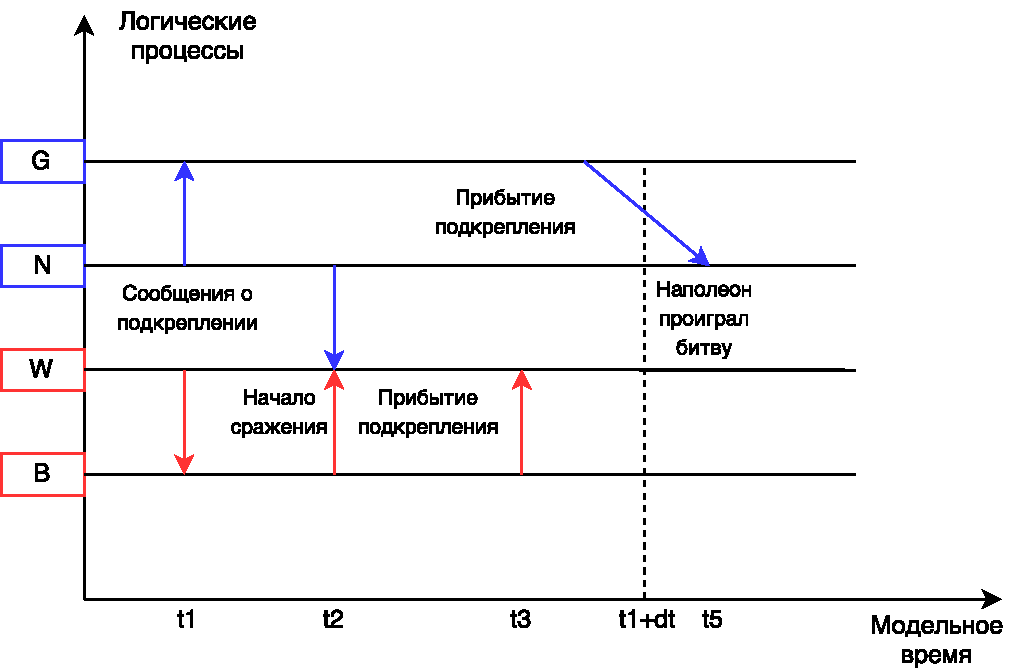
\includegraphics[scale=1]{графика/waterloo.pdf}
\caption{Корректная временная диаграмма исполнения модели}
%\label{fig:выполнение модели}
\end{figure}

Наполеон Бонапарт (процесс $N$) должен был вступить в бой с герцогом Веллингтоном (процесс $W$), расположившемся со своей английской армией на пути к Брюсселю. Но оба полководца ждали подкрепления: герцог Веллингтон --- прусского князя Блюхера (процесс $B$), Наполеон --- своего маршала Груш\'и (процесс $G$). И Наполеон и Веллингтон отправили командующим своими подкреплениями сообщения с категорическим требованием скорейшего прибытия под Ватерлоо для усиления основной группировки войск. Тем временем, армия Бонапарта в ожидании прибытия подкрепления маршала Груши начала атаку неприятеля. Веллингтону ничего не оставалось, как принять бой. Не смотря на более выгодное расположение войск Веллингтона и примерно равные силы с Наполеоном, французы развивали успешное наступление на англичан и едва не опрокинули их --- положение Веллингтона становилось критическим. И только вовремя подоспевшее подкрепление князя Блюхера помогло герцогу сдержать натиск Наполеона, а затем и перейти в контрнаступление на французов. После чего, так и не дождавшийся своего маршала с подкреплением, французский император был разбит.

Предположим, что эти процессы выполняются на распределенной системе. И логический процесс $B$ в силу определенных причин (например, резко возросла нагрузка на процессор) выполняется медленнее. Следовательно возникли задержки. Для логического процесса $W$ получение сообщения в момент времени $t5$ означает изменение прошлого в момент времени $t4$, что нарушает корректную последовательность развития моделирования.

\begin{figure}[H]
\centering
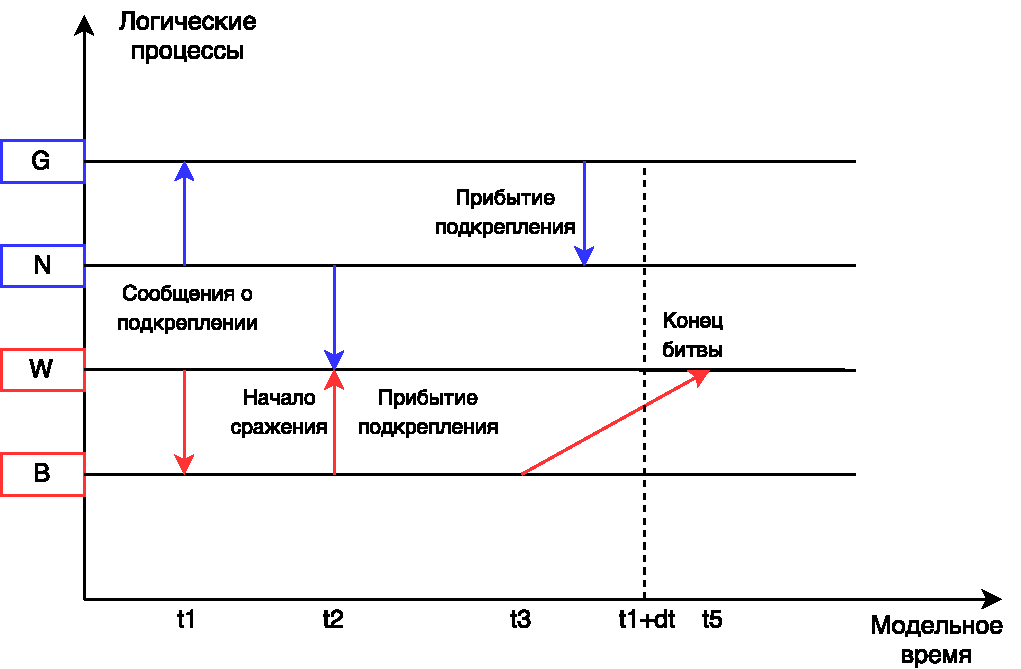
\includegraphics[scale=1]{графика/unwaterloo.pdf}
\caption{Некорректная временная диаграмма исполнения модели}
%\label{fig:выполнение модели}
\end{figure}

Для того, чтобы модель правильно воспроизводила последовательность событий в моделируемой системе, необходимо чтобы не возникало подобных парадоксов времени.
Тот процесс продвигает свое время вперед, который получил сообщение от процесса с б\'ольшим временем. Если процесс получает сообщение от процесса с меньшим временем, т.е. $t_i^m<t_i^n, \, m \to n$, получаем парадокс, т.е. говорят, что процесс приславший сообщение \elki{из прошлого} отстает во времени~\cite{okol}.

Для того, чтобы парадоксов времени в системе не возникало, необходимо предусмотреть специальные программы, которые бы синхронизировали по времени процессы в моделируемой системе. Такие программы получили название алгоритмов синхронизации модельного времени. Алгоритмы синхронизации разнообразны, но все их как правило можно разделить на два основных класса: консервативные и оптимистические.

Если синхронизация модельного времени процессов происходит под управлением консервативного алгоритма, это предполагает, что процесс получает сообщения в том же порядке, в котором их посылает ему отправитель.
Иначе, консервативные алгоритмы блокируют продвижение модельного времени в том случае, если процесс получил сообщение от процесса с меньшим временем.

Оптимистические алгоритмы в аналогичном случае осуществляют откат времени процесса с большим временем до времени процесса, приславшего сообщение, обрабатывает его, а так же заново обрабатывают все сообщения от этого времени до текущего в правильной временной последовательности.


Математическая модель консервативного алгоритма синхронизации может быть представлена в виде \cite{voz-disser}:
\begin{equation}
\label{eq:АС с синхронизацией взаимодействий}
\left\{
\begin{aligned}
x_{i+1}^n & = x_i^n + \xi_i^n F^n(i)\\
F^n(i) & = \begin{cases}
 1, & \text{если $\forall m \in M^n : x_i^n + \xi_i^n \leqslant x_i^m + \xi_i^m$} \\
 0, & \text{иначе}
 \end{cases}\\
x_0^n & = 0\\
n & = \overline{1, N}
\end{aligned}
\right.
\end{equation}
где $x_{i+1}^n$ --- время процесса $n$ на следующем шаге, $\xi_i^n$ --- локальное приращение времени процесса $n$ (время, затрачиваемое процессом на внутреннюю работу), $n$ --- процесс, который продвигает время (получает сообщение от процесса $m$), $m$ --- процесс, посылающий сообщение процессу $n$.
Поскольку общее модельное время $T_I$ --- случайная величина, будем искать ее математическое ожидание. Модельное время всей системы на $i$-ом шаге равно минимальному времени процесса на этом шаге: $\forall\,i: M(T_i)=M(x_i)$. 
\todo{Доказать оценку матожидания}
С учетом оценки математических ожиданий величин $\{x_i^{n}\}$, получаем:
\begin{equation}
\label{eq:АС с синхронизацией взаимодействий}
K^n(i)=
\left\{
\begin{aligned}
\overline{M}(x_{i+1}^n) & = \overline{M}(x_i^n) + M(\xi_i^n) \overline{F^n}(i)\\
\overline{F^n}(i) & = \begin{cases}
 1, & \text{если 
 %$\forall m \in M^n : 
 $\overline{M}(x_i^n) + M(\xi_i^n) \leqslant \overline{M}(x_i^m) + M(\xi_i^m$)} \\
 0, & \text{иначе}
 \end{cases}\\
M(x_0^n) & = 0\\
n & = \overline{1, N}
\end{aligned}
\right.
\end{equation}
  
Математическая модель оптимистического алгоритма может быть представлена в виде:
\begin{equation}
\label{eq:АС с синхронизацией взаимодействий}
\left\{
\begin{aligned}
x_{i+1}^n & = x_i^n + \xi_i^n-\max\limits_{m=\overline{1, N}}((x_i^n-x_i^m)I_i^{m\rightarrow n}I_i^{x_i^m<x_i^n})\\
x_0^n & = 0\\
n & = \overline{1, N}
\end{aligned}
\right.
\end{equation}
где $I_i^{m\rightarrow n}$ --- событие, означающее посылку сообщения процессом $m$ процессу $n$, $I_i^{x_i^m<x_i^n}$ --- событие, означающее, что время процесса $m$ меньше времени процесса $n$.

Если обозначить $\rho_i^{mn}=(x_i^n-x_i^m)I_i^{x_i^m<x_i^n}$, $\alpha_i^{mn}=I_i^{m\rightarrow n}$ получим следующую форму записи:
\begin{equation}
\label{eq:АС с синхронизацией взаимодействий}
\left\{
\begin{aligned}
x_{i+1}^n & = x_i^n + \xi_i^n-\max\limits_{m=\overline{1, N}}(\alpha_i^{mn}\rho_i^{mn})\\
x_0^n & = 0\\
n & = \overline{1, N}
\end{aligned}
\right.
\end{equation}
С учетом оценки математических ожиданий величин $\{x_i^{n}\}$, получим:
\begin{equation}
\label{eq:АС с синхронизацией взаимодействий}
O^n(i)=
\left\{
\begin{aligned}
\overline{M}(x_{i+1}^n) & = \overline{M}(x_i^n) + M(\xi_i^n)-\max\limits_{m=\overline{1, N}}(\alpha_i^{mn}\overline{M}(\rho_i^{mn}))\\
\overline{M}(\rho_i^{mn}) & = \begin{cases}
\overline{M}(x_i^n)-\overline{M}(x_i^m), & \text{если $\overline{M}(x_i^n)>\overline{M}(x_i^m)$} \\
 0, & \text{если $\overline{M}(x_i^n)\leqslant\overline{M}(x_i^m)$}
 \end{cases}\\
M(x_0^n) & = 0\\
n & = \overline{1, N}
\end{aligned}
\right.
\end{equation}

Оба приведенных алгоритма синхронизации обладают определенными недостатками: консервативный алгоритм допускает <<простои>> модельного времени процессов, оптимистический --- <<откаты>> модельного времени.

Для уменьшения количества простоев и откатов модельного времени разработан алгоритм выбора оптимальной синхронизации процессов, основанный на анализе продвижения модельного времени каждым процессом.

Начало моделирования происходит под управлением консервативного алгоритма. Продвижение времени каждого процесса, участвующего в моделировании, оценивается на предмет изменения приращения его локального времени, а так же интенсивности посылки этим процессом сообщений другим процессам, участвующим в моделировании.

\todo{Ознакомиться с источниками, по типам моделей, включить их в список литературы}

Согласно \cite{voz-disser} процессы можно условно разделить на три типа: 
\begin{enumerate}
  \item Тип 1. Математические ожидания приращений локальных часов имеют небольшой разброс \hbox{$\leqslant \hss 50\%$}, процессы активно обмениваются сообщениями \hbox{$\alpha^{mn} \hss \rightarrow \hss 1$}. К данному типу могут быть отнесены имитационные модели сетей, многопроцессорных систем обработки сигналов и любого коммуникационного оборудования.
  \item Тип 2. Математические ожидания приращений локального времени имеют неограниченный разброс, процессы довольно редко обмениваются сообщениями \hbox{$\alpha^{mn} \hss < \hss 0.5$}. Данному типу соответствуют имитационные модели работы сложных параллельных алгоритмов, где процессы в основном заняты своими внутренними вычислениями и обмениваются только входными данными и результатами. К этому типу могут относиться, например, имитационные модели алгоритмов бортового вычислительного комплекса летательного аппарата.
  \item Тип 3. Разброс математических ожиданий неограничен, процессы обмениваются сообщениями с разной интенсивностью. К такому типу можно отнести полные модели распределенных вычислительных систем, например имитационная модель бортового навигационного комплекса.
\end{enumerate}

Там же, в ходе экспериментов было установлено, что в зависимости от распределения приращений локальных часов можно говорить о наибольшей эффективности какого-либо алгоритма синхронизации для определенного типа процесса.

В общем виде алгоритм выбора оптимальной синхронизации следующий.
\begin{itemize}


\item[Шаг\;1.] Ввод исходных данных: число процессов, участвующих в моделировании, число шагов моделирования, вероятность посылки сообщений процессами лежит в интервале от 0 до 1, разброс приращений локальных часов --- неограничен.

\item[Шаг\;2.] Старт моделирования. На данном шаге генерируются последовательности посылки сообщений каждым процессом и приращения локального времени для процесса. 

\item[Шаг\;3.] Процессы в соответствии с последовательностями обмениваются сообщениями. Продвижение времени происходит по консервативному алгоритму.

\item[Шаг\;4.] Если заключительный шаг моделирования не достигнут, то в течение (следующих) $10$ шагов анализируются интенсивности посылки сообщений каждым процессом и величины локального приращения времени. Иначе --- моделирование заканчивается. Если пара <<\textit{вероятность посылки сообщений --- локальное приращение времени процесса}>> удовлетворяет какому-либо заданному типу, то следующие $10$ шагов процесс осуществляет продвижение времени, синхронизируя его с помощью наиболее оптимального для этой пары алгоритма синхронизации. Например, процесс посылает сообщения с интенсивностью 6 сообщений за 10 шагов. Это означает, что вероятность посылки составляет $0.6$. Если приращение локального времени процесса в результате получения сообщений от других процессов \hbox{$\leqslant \hss 50\%$}, то процесс принадлежит к типу $1$. Для данного типа процессов наиболее эффективен консервативный алгоритм синхронизации. Это означает, что следующие $10$ шагов процесс будет продвигать свое время с помощью консервативного алгоритма. Если один из параметров процесса указывает на его принадлежность к типу $2$, то наиболее оптимальным алгоритмом синхронизации для процесса будет оптимистический и следующие $10$ шагов процесс будет продвигать свое время с помощью этого алгоритма.

\item[Шаг 5.] Переход на Шаг 4.

\end{itemize}

Обозначим $\Theta^n(i)$ функцию, меняющую свое значение в зависимости от типа процесса

\begin{equation}
\label{eq:АС с синхронизацией взаимодействий}
\overline\Theta^n(i)=
\left.
\begin{cases}
 1, & \text{если
 %$\forall m \in M^n : 
 $\alpha^{mn}\rightarrow 1$, \,$\Delta T \leqslant 50\%$} \\
 0, & \text{если
 $\alpha^{mn} < 0.5, \, \Delta T \rightarrow\infty$} \\
  & \text{если
 $\alpha^{mn}\in [0\ldots1], \, \Delta T \in[0\ldots \infty]$} \\
m,\;n & = \overline{1, N}
\end{cases}
\right.
\end{equation}

где $\Delta T$ --- относительное приращение локального времени процессом.

\begin{equation}
\begin{aligned}
\Delta T_{\text{отн.}}= \frac{\Delta T_{\text{абс.}}}{min\,M(\xi_i^n)}100\%\,,
\\
\Delta T_{\text{абс.}}=max\,M(\xi_i^n)-min\,M(\xi_i^n)\,.
\end{aligned}
\end{equation}

Математическая модель выбора оптимального алгоритма синхронизации, с учетом оценок математического ожидания, будет иметь вид:

%%% Здесь посмотреть на диссер харьковчан, как там записывается полная матмодель
%%% Разобраться с оверлайн над функциями

\begin{equation}
\label{eq:АС с синхронизацией взаимодействий}
\left\{
\begin{aligned}
\overline{M}(x_{i+1}^n) & = \overline{K^n}(i)\overline{\Theta^n}(i) + \overline{O^n}(i)\overline{\Theta^n}(i)\\
\overline{K_i^n}(i) & = \overline{M}(x_i^n) + M(\xi_i^n) \overline{F^n}(i)\\
\overline{F^n}(i) & = \begin{cases}
 1, & \text{если 
 %$\forall m \in M^n : 
 $\overline{M}(x_i^n) + M(\xi_i^n) \leqslant \overline{M}(x_i^m) + M(\xi_i^m$)} \\
 0, & \text{иначе}
 \end{cases}\\
 \overline{O_i^n}(i) & = \overline{M}(x_i^n) + M(\xi_i^n)-\max\limits_{m=\overline{1, N}}(\alpha_i^{mn}\overline{M}(\rho_i^{mn}))\\
\overline{M}(\rho_i^{mn}) & = \begin{cases}
\overline{M}(x_i^n)-\overline{M}(x_i^m), & \text{если $\overline{M}(x_i^n)>\overline{M}(x_i^m)$} \\
 0, & \text{если $\overline{M}(x_i^n)\leqslant\overline{M}(x_i^m)$}
 \end{cases}\\
\overline{\Theta^n}(i) & = \begin{cases}
1, & \text{если
 %$\forall m \in M^n : 
 $\alpha^{mn}\rightarrow 1, \, \Delta T \leqslant50\%$} \\
 0, & \text{если
 $\alpha^{mn} < 0.5, \, \Delta T \rightarrow\infty$} \\
  & \text{
 $\alpha^{mn}\in [0\ldots1], \, \Delta T \in[0\ldots \infty]$} \\
m,\;n & = \overline{1, N}
 \end{cases}\\
M(x_0^n) & = 0\\
m,\,n & = \overline{1, N}
\end{aligned}
\right.
\end{equation}

Работа алгоритма была смоделирована с применением приложения Wolfram Mathematica и показала следующие результаты (на рисунке продвижение времени оптимальным алгоритмам обозначено как <<КАС +>>).

\begin{enumerate}

\item Все процессы принадлежат 1 типу.

\begin{figure}[H]
\centering
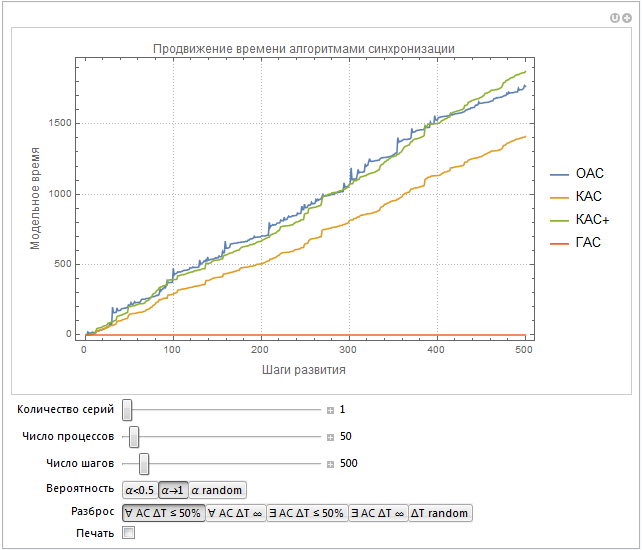
\includegraphics[scale=1]{графика/typeA.png}
\caption{Тип 1. Продвижение времени алгоритмами синхронизации}
%\label{fig:выполнение модели}
\end{figure}

\begin{figure}[H]
\centering
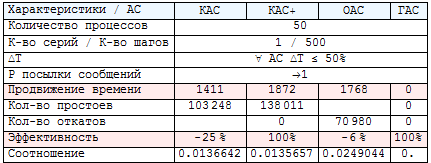
\includegraphics[scale=1]{графика/tableA.png}
\caption{Тип 1. Сравнительная эффективность алгоритмов синхронизации}
%\label{fig:выполнение модели}
\end{figure}

\item Все процессы принадлежат 2 типу.

\begin{figure}[H]
\centering
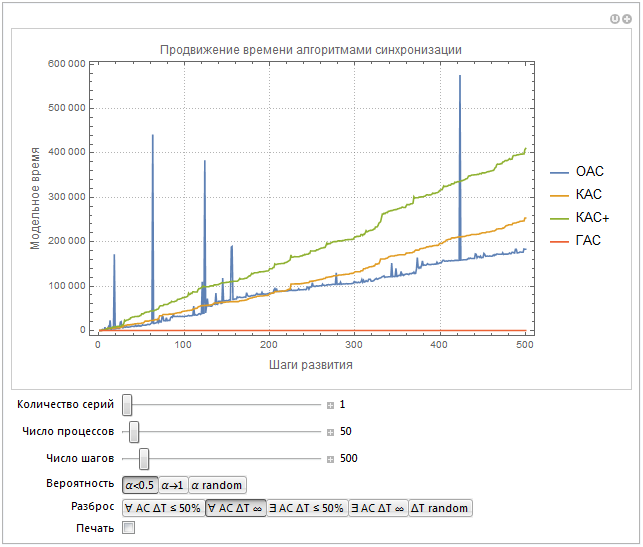
\includegraphics[scale=1]{графика/typeB.png}
\caption{Тип 2. Продвижение времени алгоритмами синхронизации}
%\label{fig:выполнение модели}
\end{figure}

\begin{figure}[H]
\centering
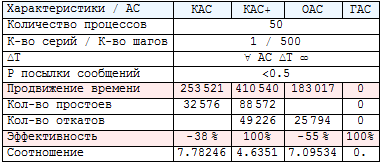
\includegraphics[scale=1]{графика/tableB.png}
\caption{Тип 2. Сравнительная эффективность алгоритмов синхронизации}
%\label{fig:выполнение модели}
\end{figure}

\item Процессы смешанного типа.

\begin{figure}[H]
\centering
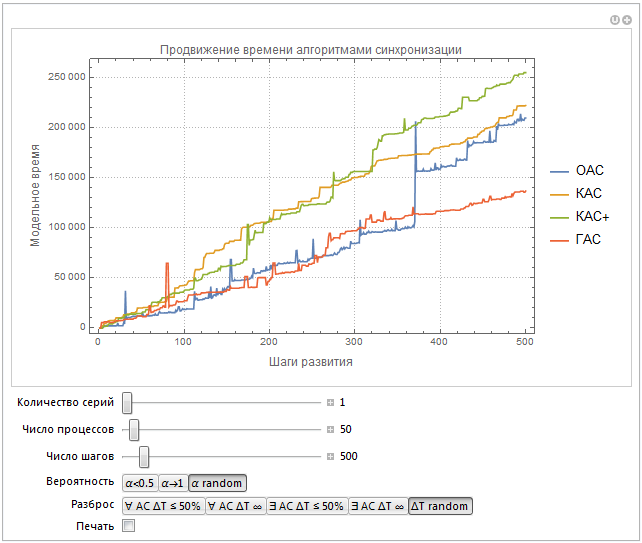
\includegraphics[scale=1]{графика/typeAB.png}
\caption{Тип 3. Продвижение времени алгоритмами синхронизации}
%\label{fig:выполнение модели}
\end{figure}

\begin{figure}[H]
\centering
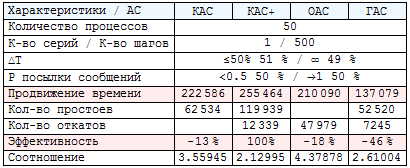
\includegraphics[scale=1]{графика/tableAB.png}
\caption{Тип 3. Сравнительная эффективность алгоритмов синхронизации}
%\label{fig:выполнение модели}
\end{figure}

\end{enumerate}


Выводы.

Эксперименты показали, что продвижение времени процессами с помощью алгоритма выбора оптимальной синхронизации для всех типов процессов дает лучший результат, чем в случае, если бы продвижение времени происходило с помощью только консервативного алгоритма или только оптимистического алгоритма синхронизации. В случае, когда синхронизация времени осуществляется для процессов типа 1, алгоритм выбора оптимальной синхронизации дает результаты едва лучшие алгоритма оптимистического. В случае, когда продвижение времени процессов осуществляется для процессов типа 2, алгоритм выбора оптимальной синхронизации показывает результаты лучшие, чем консервативный и значительно лучшие, чем оптимистический. При использовании смешанного типа процессов, алгоритм выбора оптимальной синхронизации так же способен показывать результаты, лучшие, чем алгоритмы консервативной и оптимистической синхронизации. 
\bibliography{../nir}






%\begin{figure}[H]
%\centering
%\includegraphics[scale=0.95]{}
%\caption{}
%\label{fig:выполнение модели}
%\end{figure}



\end{document}
